\documentclass{report} % change to article

\usepackage[margin=1in]{geometry}
\usepackage{url}
\usepackage{graphicx}
\usepackage{grffile}
\usepackage{caption}
\usepackage{subcaption}

\graphicspath{{../ExampleDatasets/}}
\DeclareGraphicsExtensions{.png}

\AtBeginDocument{\renewcommand{\bibname}{\Large References}}

\title{Project Report\\[0.5em]{\Large on}\\[0.5em]Finding Link Communities in Edge Attributed Networks}
\author{Data Mining\\CSCI 479\\Dr. Saeed Salem\\[1em] Joshua Tan\\joshua.tan@ndsu.edu}

\date{December 19, 2013}

\setlength\parindent{0pt}

\begin{document}
\maketitle

\section*{Introduction}


How to use edge attribute information to find communities? How does this change the types of communities identified in a network?

\section*{Related Work}

An important task in identiying communities with networks is to explicitly define what constitutes a community. A common approach is to define a community in terms of nodes and their interconnectivity; a community would correspond to a subset of nodes forming a dense subgraph in the original network. Another approach is to focus on the network links, instead of the nodes. Ahn et al. describe a method for extracting communities using this approach, and show how the resulting link communities naturally incorporate both hierarchichal organization and overlap in communities \cite{ahn-lehmann-link-communities-nature-2010}. Salem and Ozcaglar also show how dense subgraph mining can be accomplished for coexpression graphs \cite{Salem:2013:MMF:2500863.2500869}. The approach they utilize consists of two steps: in the first, maximal frequent edgesets are mined, and in the second, highly-connected subgraphs ad extracted from the resulting edge-induced subgraphs.\\

Other research has been conducted studying the role node attributes play in the formulation of communities. Silva et al. explore this topic, by analyzing the correlation between attributes sets of nodes and the occurence of dense subgraphs; they present the Structural Correlation Pattern Mining (SCPM) algorithm and demonstrate its effectiveness on large real attributed graphs \cite{DBLP:journals/corr/abs-1201-6568}.

\section*{Algorithms}

This research combines the structurual similarity of edges with the similarity of edge attribute sets for determining communities in a network. The structural similarity metric utilized corresponds to the link similarity metric used by Ahn et al. \cite{ahn-lehmann-link-communities-nature-2010}. Let $n_+(i)$ designate the set of node $i$ and its neighbors. We can then express the similarity of two edges $e_{ik}$ and $e_{jk}$ using the following equation:

\begin{equation}
  S_{struct}(e_{ik},e_{jk}) = \frac{|n_+(i) \cap n_+(j)|}{|n_+(i) \cup n_+(j)|}
\end{equation}

An additional similarity metric can be used to quantify the similarity of edges, based on their attribute sets. Let $e_i$ be the set of attributes for edge $i$. The similarity of two edges $e_{ik}$ and $e_{jk}$ is then expressed as follow:

\begin{equation}
  S_{attr}(e_{ik},e_{jk}) = \frac{|e_i \cap e_j|}{|e_i \cup e_j|}
\end{equation}

In this equation, it is important to note that edges not sharing a common node are assigned a similarity of 0, regardless of if they share attributes. We can combine these two metrics to formulate a more comprehensive similarity metric:

\begin{equation}
  S(e_{ik},e_{jk}) = \alpha (S_{struct}(e_{ik},e_{jk})) + (1-\alpha)(S_{attr}(e_{ik},e_{jk}))
\end{equation}

The specific value of $\alpha$ will determine the proportion of the final similarity measure that either components contributes.

\section*{Experimental Results}

Two scripts were developed to conduct experiments using the approach developed in this research. A Python script is used to calculate edge attribute similarities, and an R script combined this measurement with information on structural similarity for edges. The R script also performs the clustering and visualization tasks, using the R \texttt{igraph} package\footnote{http://igraph.sourceforge.net/}. Both scripts made heavy use of a set of programs provided by Ahn et al.\footnote{http://barabasilab.neu.edu/projects/linkcommunities/}. These scripts are available as open-source\footnote{https://github.com/jtan189/linkcomm}.\\

Using these scripts, two toy networks are clustered\footnote{Due to memory issues, it was not possible to test this new metric out on the real DBLP dataset. In the future, this could be accomplished by translating the existing Python script to a more efficient C++ script.}. Each toy network was designed to test out of different network community scenarios.

\subsection*{Network \#1}

Network \#1 was designed to test the case where two dense subgraphs exist in a network, but within those subgraphs, the attributes for the connecting edges are nonhomogeneous. Figure~\ref{fig:net1_orig} shows the graph for this network, before clustering.

\begin{figure}[htp!]
  \centering
  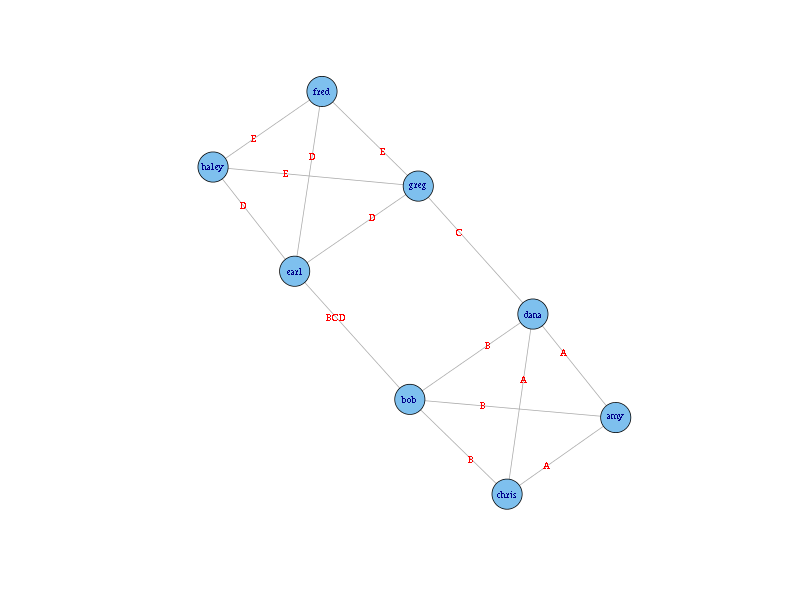
\includegraphics[width=0.55\linewidth]{toy2/orig.png}
  \caption{Original graph for Network \#1.}
  \label{fig:net1_orig}
\end{figure}

The results of clustering Network \#1 are shown in Figure~\ref{fig:net1_comm}, using both types of similarity metrics.\\

\begin{figure}[htp!]
  \centering
  \begin{subfigure}{.5\textwidth}
    \centering
    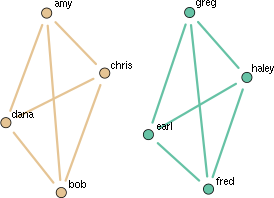
\includegraphics[width=.8\linewidth]{toy2/no_ea/edge_comm.png}
    \caption{Using structural similarity only.}
    \label{fig:net1_comm_struct}
  \end{subfigure}%
  \begin{subfigure}{.5\textwidth}
    \centering
    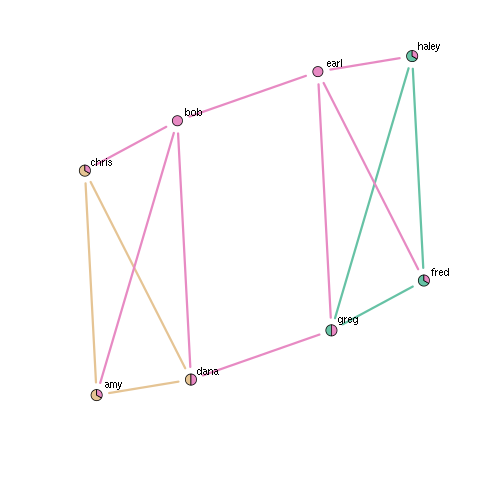
\includegraphics[width=.9\linewidth]{toy2/ea/edge_comm_0.1.png}
    \caption{Using both, 10\% structural.}
    \label{fig:net1_comm_both_10}
  \end{subfigure}
  \caption{Communities extracted from Network \#1.}
  \label{fig:net1_comm}
\end{figure}

From Figure~\ref{fig:net1_comm}, we can see the effectivieness of the combined similarity metric in identifying communities based on edge attributes. Using structural similarity only, \textit{bob} iis clustered together with \textit{amy}, \textit{chris}, and \textit{dana}, even though his edges to the other three nodes have distinct attributes from the edges interconnecting these other three nodes. By placing a greater emphasis on edge attributes in determining edge similarity, the combined approach is able to identify this distinction.\\

Using Network \#1, it is also clear the effect that the chosen $\alpha$ value can have on the resulting clustering. By increase $\alpha$ from 0.1 to 0.25 (corresponding to a similarity measure this is 25\% structural and 75\% attribute-based), a different clustering is produced (Figure~\ref{fig:net1_comm_both_25}).\\
% \begin{figure}[htp!]
%   \centering
%   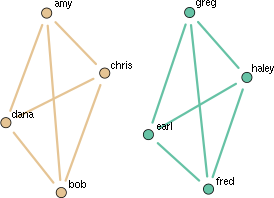
\includegraphics[width=0.65\linewidth]{toy2/no_ea/edge_comm.png}
%   \caption{Communities using structural similarity only.}
% \end{figure}

% \begin{figure}[htp!]
%   \centering
%   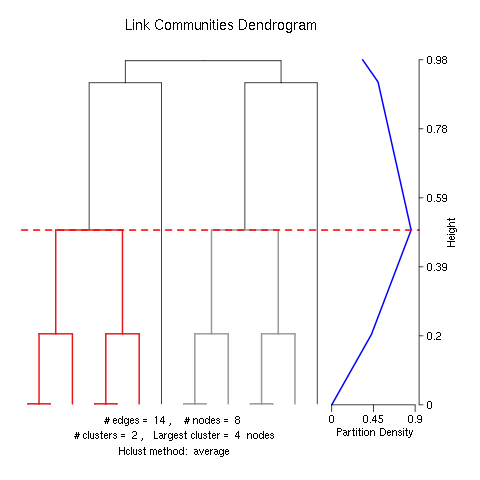
\includegraphics[width=0.65\linewidth]{toy2/no_ea/lc.png}
%   \caption{Link communities dendogram using structural similarity only.}
% \end{figure}

% \begin{figure}[htp!]
%   \centering
%   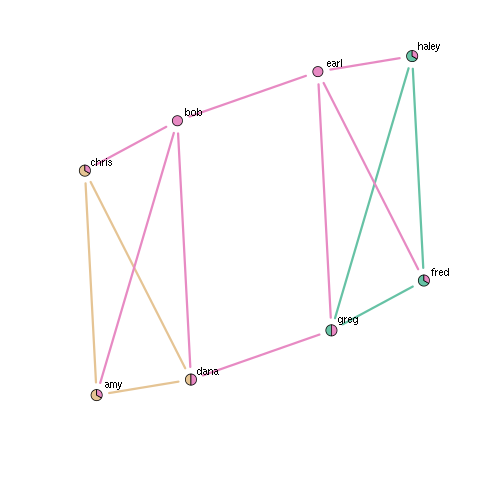
\includegraphics[width=0.65\linewidth]{toy2/ea/edge_comm_0.1.png}
%   \caption{Communities using both, 10 percent structural.}
% \end{figure}

\begin{figure}[htp!]
  \centering
  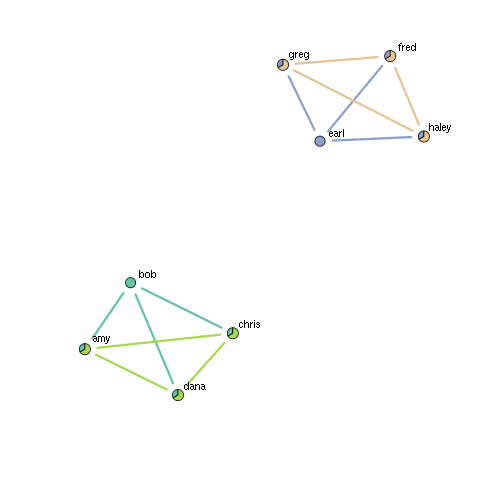
\includegraphics[width=0.5\linewidth]{toy2/ea/edge_comm_0.25.png}
  \caption{Communities for Network \#1. Using both, 25\% structural.}
  \label{fig:net1_comm_both_25}
\end{figure}

Figures~\ref{fig:net1_dend_10} and \ref{fig:net1_dend_25} elucidate the reason for these differences. Although both the community dendograms for both networks contain the same structure, in the combined similarity approach, the partition density is weakened by the merging \textit{bob} and \textit{earl} into a larger community. This is due to less emphasis being placed on the fact that the edges \textit{bob-earl} and \textit{dana-greg} share attributes with the edges in smaller communites they join. Since the cutoff threshold used to identify significant communities is based on the maximum partition density, the largest community in \ref{fig:net1_comm_both_10} is divided into two communities in \ref{fig:net1_comm_both_25}.\\

\begin{figure}[htp!]
  \centering
  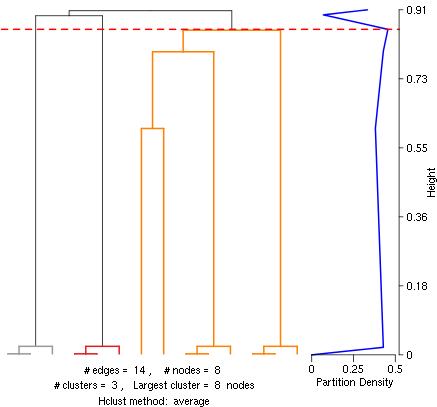
\includegraphics[width=0.5\linewidth]{toy2/ea/lc_0.1.png}
  \caption{Link communities dendogram for Network \#1. Using both, 10\% structural.}
  \label{fig:net1_dend_10}
\end{figure}

\begin{figure}[htp!]
  \centering
  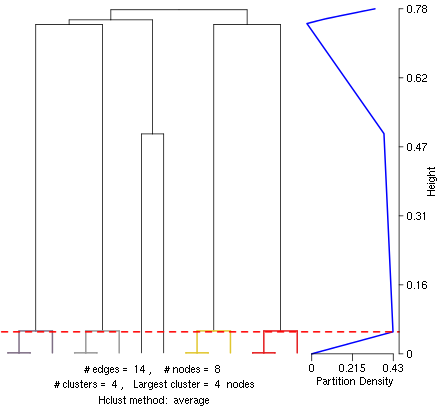
\includegraphics[width=0.5\linewidth]{toy2/ea/lc_0.25.png}
  \caption{Link communities dendogram for Network \# 1. Using both, 25\% structural.}
  \label{fig:net1_dend_25}
\end{figure}

Figure~\ref{fig:net1_member} clearly identifies the communites each node is a part of, while also demonstrating the hierarchical overlap between certain communities.\\

\begin{figure}[htp!]
  \centering
  \begin{subfigure}{.4\textwidth}
    \centering
    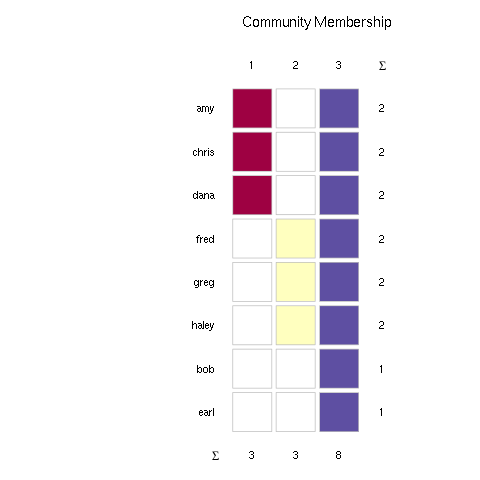
\includegraphics[width=.6\linewidth]{toy2/ea/top20_0.1.png}
    \caption{Using both, 10\% structural.}
    \label{fig:net1_member_struct}
  \end{subfigure}%
  \begin{subfigure}{.6\textwidth}
    \centering
    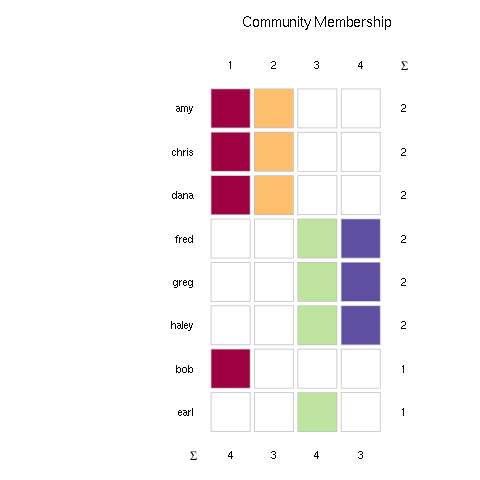
\includegraphics[width=.6\linewidth]{toy2/ea/top20_0.25.png}
    \caption{Using both, 25\% structural.}
    \label{fig:net1_member_both}
  \end{subfigure}
  \caption{Community membership for Network \#1.}
  \label{fig:net1_member}
\end{figure}

% \begin{figure}[htp!]
%   \centering
%   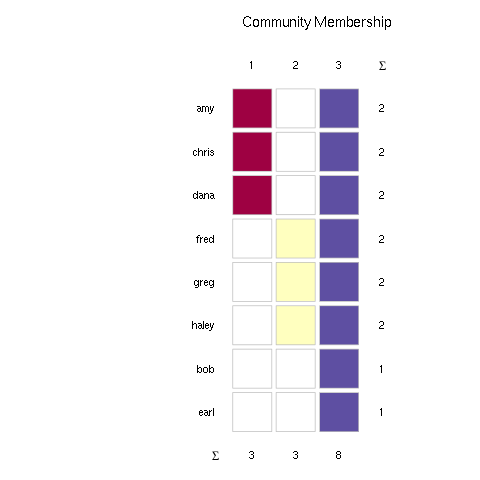
\includegraphics[width=0.65\linewidth]{toy2/ea/top20_0.1.png}
%   \caption{Community membership using both, 10 percent structural.}
% \end{figure}

% \begin{figure}[htp!]
%   \centering
%   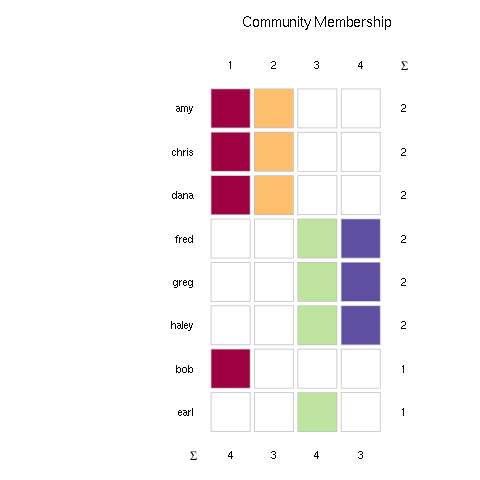
\includegraphics[width=0.65\linewidth]{toy2/ea/top20_0.25.png}
%   \caption{Community membership using both, 25 percent structural.}
% \end{figure}

\newpage

\subsection*{Network \#2}

Network \#2 presents an example where two distinct nodes can be divided into three distinct groups, based on edge attributes. However, the subgraphs associated with these groups are not dense. Figure~\ref{fig:net2_orig} shows the graph for for this network.

\begin{figure}[htp!]
  \centering
  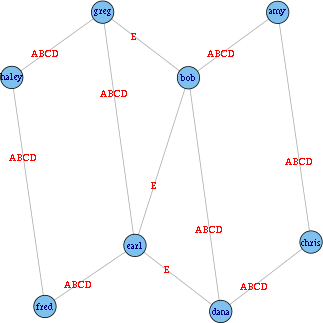
\includegraphics[width=0.5\linewidth]{toy3/orig.png}
  \caption{Original graph for toy Dataset \#2.}
  \label{fig:net2_orig}
\end{figure}

As before, this network is clustered using the approach where only structural similarities are considered, and the approach where both structural and edge attribute similarity are considered (Figure~\ref{fig:net2_comm}).\\

\begin{figure}[htp!]
  \centering
  \begin{subfigure}{.5\textwidth}
    \centering
    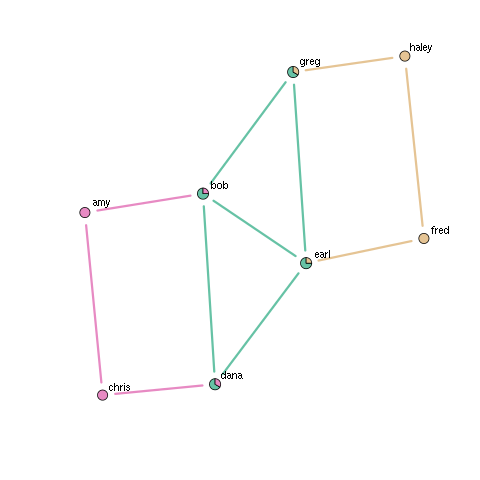
\includegraphics[width=.8\linewidth]{toy3/no_ea/edge_comm.png}
    \caption{Using structural similarity only.}
    \label{fig:net2_comm_struct}
  \end{subfigure}%
  \begin{subfigure}{.5\textwidth}
    \centering
    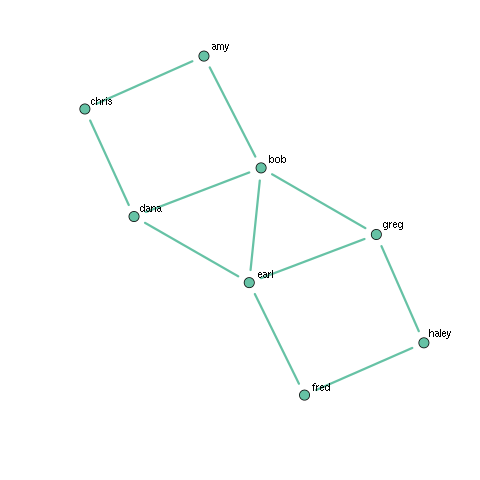
\includegraphics[width=.9\linewidth]{toy3/ea/edge_comm_0.25.png}
    \caption{Using both. Unchanged from 10\% to 90\%.}
    \label{fig:net2_comm_both}
  \end{subfigure}
  \caption{Communities extracted from Network \#2.}
  \label{fig:net2_comm}
\end{figure}

The results of these clusterings may seem unintuitive. As expected, Figure~\ref{fig:net2_comm_struct} shows clusters that are not homogeneous with respect to attributes. However, the combined similarity approach fails to find any distinct communities with the network. Based on shared edge attributes, we might expect the sets \{\textit{amy}, \textit{bob}, \textit{chris}, \textit{dana}\} and \{\textit{earl}, \textit{fred}, \textit{greg}, \textit{haley}\} to belong to the same community. However, since these two communities are separated by edges that only contain the attribute \textit{E}, the combined similarity algorithm the attribute similarity between edges in these two components to be zero. This is a result of the implementation decision requiring edges to directly share a common node in order to be assigned a nonzero attribute similarity. \\

The community dendogram in Figure~\ref{fig:net2_dend} illustrates how the partition density for the decreases as additional partitions (communities) are introduced.

% \begin{figure}[htp!]
%   \centering
%   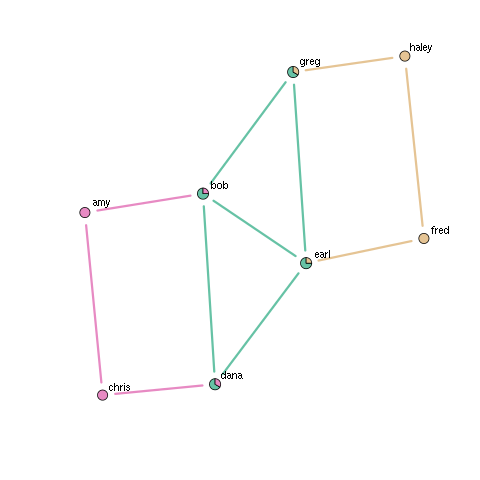
\includegraphics[width=0.65\linewidth]{toy3/no_ea/edge_comm.png}
%   \caption{Communities using structural similarity only.}
% \end{figure}

% \begin{figure}[htp!]
%   \centering
%   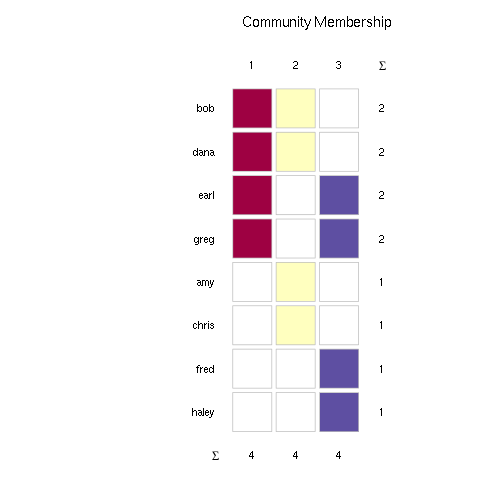
\includegraphics[width=0.3\linewidth]{toy3/no_ea/top20.png}
%   \caption{Community membership for Network \#2. Using structural similarity only.}
% \end{figure}

% \begin{figure}[htp!]
%   \centering
%   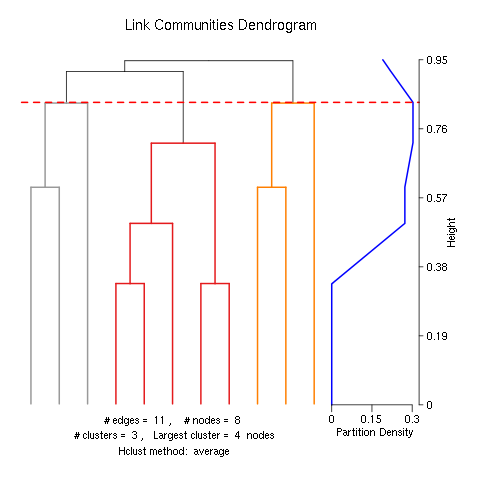
\includegraphics[width=0.6\linewidth]{toy3/no_ea/lc.png}
%   \caption{Link communities dendogram for Network \#2. Using structural similarity only.}
% \end{figure}

\begin{figure}[htp!]
  \centering
  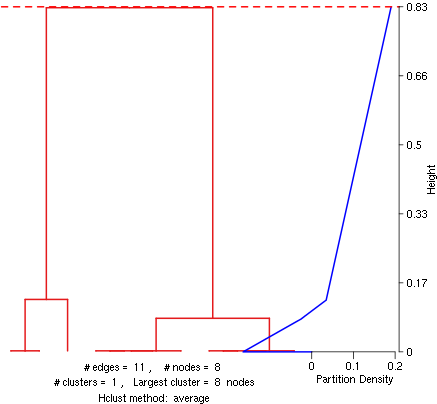
\includegraphics[width=0.5\linewidth]{toy3/ea/lc_0.25.png}
  \caption{Link communities dendogram for Network \#2. Using both, 25\% structural.}
  \label{fig:net2_dend}
\end{figure}

% \begin{figure}[htp!]
%   \centering
%   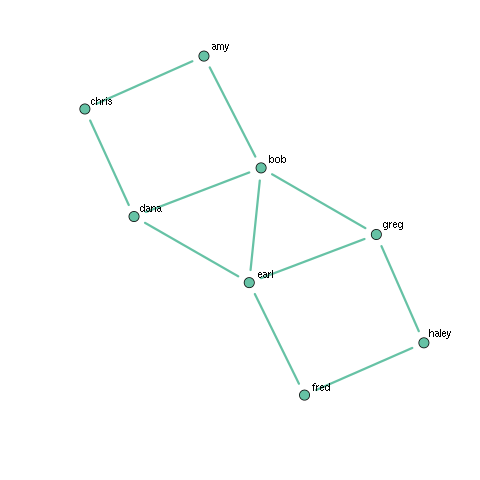
\includegraphics[width=0.65\linewidth]{toy3/ea/edge_comm_0.25.png}
%   \caption{Communities using both. Unchanged from 10\% to 90\%.}
% \end{figure}

\section*{Conclusions}

New approach may be appropriate if wish to cluster according to both link structure and edge attributes.\\

Limitations: In some cases, result is highly depend on chosen alpha value. In others, edge attributes are more influential in similarity measure, despite chosen alpha value. In both cases, it is necessary to choose the cutoff threshold for determining communities.
Implementation

\bibliography{references}
\bibliographystyle{unsrt}

\end{document}

%%% Local Variables: 
%%% mode: latex
%%% TeX-master: t
%%% End: 
